\documentclass[12pt, titlepage]{article}

\usepackage{fullpage}
\usepackage[round]{natbib}
\usepackage{multirow}
\usepackage{booktabs}
\usepackage{tabularx}
\usepackage{graphicx}
\usepackage{float}
\usepackage{hyperref}
\hypersetup{
    colorlinks,
    citecolor=blue,
    filecolor=black,
    linkcolor=red,
    urlcolor=blue
}

%% Comments

\usepackage{color}

\newif\ifcomments\commentstrue %displays comments
%\newif\ifcomments\commentsfalse %so that comments do not display

\ifcomments
\newcommand{\authornote}[3]{\textcolor{#1}{[#3 ---#2]}}
\newcommand{\todo}[1]{\textcolor{red}{[TODO: #1]}}
\else
\newcommand{\authornote}[3]{}
\newcommand{\todo}[1]{}
\fi

\newcommand{\wss}[1]{\authornote{blue}{SS}{#1}} 
\newcommand{\plt}[1]{\authornote{magenta}{TPLT}{#1}} %For explanation of the template
\newcommand{\an}[1]{\authornote{cyan}{Author}{#1}}

%% Common Parts

\newcommand{\progname}{ProgName} % PUT YOUR PROGRAM NAME HERE
\newcommand{\authname}{Team \#, Team Name
\\ Student 1 name
\\ Student 2 name
\\ Student 3 name
\\ Student 4 name} % AUTHOR NAMES                  

\usepackage{hyperref}
    \hypersetup{colorlinks=true, linkcolor=blue, citecolor=blue, filecolor=blue,
                urlcolor=blue, unicode=false}
    \urlstyle{same}
                                


\newcounter{acnum}
\newcommand{\actheacnum}{AC\theacnum}
\newcommand{\acref}[1]{AC\ref{#1}}

\newcounter{ucnum}
\newcommand{\uctheucnum}{UC\theucnum}
\newcommand{\uref}[1]{UC\ref{#1}}

\newcounter{mnum}
\newcommand{\mthemnum}{M\themnum}
\newcommand{\mref}[1]{M\ref{#1}}

\begin{document}

\title{Module Guide for BrainInsight3D: 3D fMRI
  Visualization \& Segmentation}
\author{Nada Elmasry}
\date{\today}

\maketitle

\pagenumbering{roman}

\section{Revision History}

\begin{tabularx}{\textwidth}{p{3cm}p{2cm}X}
  \toprule {\bf Date} & {\bf Version} & {\bf Notes} \\
  \midrule
  Date 1              & 1.0           & Notes       \\
  Date 2              & 1.1           & Notes       \\
  \bottomrule
\end{tabularx}

\newpage

\section{Reference Material}

This section records information for easy reference.

\subsection{Abbreviations and Acronyms}

\renewcommand{\arraystretch}{1.2}
\begin{tabular}{l l}
  \toprule
  \textbf{symbol} & \textbf{description}                \\
  \midrule
  AC              & Anticipated Change                  \\
  DAG             & Directed Acyclic Graph              \\
  M               & Module                              \\
  MG              & Module Guide                        \\
  OS              & Operating System                    \\
  R               & Requirement                         \\
  SC              & Scientific Computing                \\
  SRS             & Software Requirements Specification \\
  \progname       & Explanation of program name         \\
  UC              & Unlikely Change                     \\

  \bottomrule
\end{tabular}\\

\newpage

\tableofcontents

\listoftables

\listoffigures

\newpage

\pagenumbering{arabic}

\section{Introduction}

Decomposing a system into modules is a commonly accepted approach to developing
software.  A module is a work assignment for a programmer or programming
team~\citep{ParnasEtAl1984}.  We advocate a decomposition
based on the principle of information hiding~\citep{Parnas1972a}.  This
principle supports design for change, because the ``secrets'' that each module
hides represent likely future changes.  Design for change is valuable in SC,
where modifications are frequent, especially during initial development as the
solution space is explored.

Our design follows the rules layed out by \citet{ParnasEtAl1984}, as follows:
\begin{itemize}
  \item System details that are likely to change independently should be the
        secrets of separate modules.
  \item Each data structure is implemented in only one module.
  \item Any other program that requires information stored in a module's data
        structures must obtain it by calling access programs belonging to that module.
\end{itemize}

After completing the first stage of the design, the Software Requirements
Specification (SRS), the Module Guide (MG) is developed~\citep{ParnasEtAl1984}. The MG
specifies the modular structure of the system and is intended to allow both
designers and maintainers to easily identify the parts of the software.  The
potential readers of this document are as follows:

\begin{itemize}
  \item New project members: This document can be a guide for a new project member
        to easily understand the overall structure and quickly find the
        relevant modules they are searching for.
  \item Maintainers: The hierarchical structure of the module guide improves the
        maintainers' understanding when they need to make changes to the system. It is
        important for a maintainer to update the relevant sections of the document
        after changes have been made.
  \item Designers: Once the module guide has been written, it can be used to
        check for consistency, feasibility, and flexibility. Designers can verify the
        system in various ways, such as consistency among modules, feasibility of the
        decomposition, and flexibility of the design.
\end{itemize}

The rest of the document is organized as follows. Section
\ref{SecChange} lists the anticipated and unlikely changes of the software
requirements. Section \ref{SecMH} summarizes the module decomposition that
was constructed according to the likely changes. Section \ref{SecConnection}
specifies the connections between the software requirements and the
modules. Section \ref{SecMD} gives a detailed description of the
modules. Section \ref{SecTM} includes two traceability matrices. One checks
the completeness of the design against the requirements provided in the SRS. The
other shows the relation between anticipated changes and the modules. Section
\ref{SecUse} describes the use relation between modules.

\section{Anticipated and Unlikely Changes} \label{SecChange}

This section lists possible changes to the system. According to the likeliness
of the change, the possible changes are classified into two
categories. Anticipated changes are listed in Section \ref{SecAchange}, and
unlikely changes are listed in Section \ref{SecUchange}.

\subsection{Anticipated Changes} \label{SecAchange}

Anticipated changes are the source of the information that is to be hidden
inside the modules. Ideally, changing one of the anticipated changes will only
require changing the one module that hides the associated decision. The approach
adapted here is called design for
change.

\begin{description}
  \item[\refstepcounter{acnum} \actheacnum \label{acSeg}:] The segmentation algorithm
        can change after experimentation and evaluation of accuracy and speed of inference.
  \item[\refstepcounter{acnum} \actheacnum \label{acProc}:] The image processing steps can
        can change and some steps may be omitted after evaluation of performance and speed to
        reach the best performance at the fastest speed.
  \item[\refstepcounter{acnum} \actheacnum \label{acInputFormat}:] Additional input formats as DICOM
        maybe supported based on time limitations.
  \item[\refstepcounter{acnum} \actheacnum \label{acUI}:] User Interface Design and Functionality can change
        if better design and functionality were discovered while in development process.
\end{description}

\subsection{Unlikely Changes} \label{SecUchange}

The module design should be as general as possible. However, a general system is
more complex. Sometimes this complexity is not necessary. Fixing some design
decisions at the system architecture stage can simplify the software design. If
these decision should later need to be changed, then many parts of the design
will potentially need to be modified. Hence, it is not intended that these
decisions will be changed.

\begin{description}
  \item[\refstepcounter{ucnum} \uctheucnum \label{ucInputType}:] The application is
        unlikely to support other types of fMRI scans as neck and bones as they require different segmentation algorithms
        and substantial effort.
  \item [\refstepcounter{ucnum} \uctheucnum \label{ucSeg}:] The addition of functional segmentation.
  \item [\refstepcounter{ucnum} \uctheucnum \label{ucArch}:] The system main architecture and modules interaction and flow
        steps are unlikely to change as they are the foundational steps in image processing and segmentation.
\end{description}

\section{Module Hierarchy} \label{SecMH}

This section provides an overview of the module design. Modules are summarized
in a hierarchy decomposed by secrets in Table \ref{TblMH}. The modules listed
below, which are leaves in the hierarchy tree, are the modules that will
actually be implemented.

\begin{description}
  \item [\refstepcounter{mnum} \mthemnum \label{mHH}:] Hardware-Hiding Module
  \item [\refstepcounter{mnum} \mthemnum \label{mIF}:] Input Format Module
  \item [\refstepcounter{mnum} \mthemnum \label{mIV}:] Input Verification Module
  \item [\refstepcounter{mnum} \mthemnum \label{mDP}:] Data Preprocessing Module

  \item [\refstepcounter{mnum} \mthemnum \label{m2DS}:] 2D Slice Module

  \item [\refstepcounter{mnum} \mthemnum \label{m3DV}:] 3D Volume Module

  \item [\refstepcounter{mnum} \mthemnum \label{mSeg}:] Segmentation Module

  \item [\refstepcounter{mnum} \mthemnum \label{mUI}:] User Interface Module

  \item [\refstepcounter{mnum} \mthemnum \label{mMP}:] Main Program Module

  \item [\refstepcounter{mnum} \mthemnum \label{m2DDV}:] 2D Data Visualization Module
  \item [\refstepcounter{mnum} \mthemnum \label{m3DDV}:] 3D Data Visualization Module

  \item [\refstepcounter{mnum} \mthemnum \label{mUIR}:] User Interface Rendering Module
  \item [\refstepcounter{mnum} \mthemnum \label{mSegP}:] Segmentation Algorithm Processing Module
  \item [\refstepcounter{mnum} \mthemnum \label{mOp}:] Optimization Module

\end{description}


\begin{table}[h!]
  \centering
  \begin{tabular}{p{0.3\textwidth} p{0.6\textwidth}}
    \toprule
    \textbf{Level 1}                                      & \textbf{Level 2}                         \\
    \midrule

    {Hardware-Hiding Module}                              & ~                                        \\
    \midrule

    \multirow{7}{0.3\textwidth}{Behaviour-Hiding Module}  & Input Format Module                      \\
                                                          & Input Verification Module                \\
                                                          & Data Preprocessing Module                \\
                                                          & 2D Slice Module                          \\
                                                          & 3D Volume Module                         \\
                                                          & Segmentation Module                      \\
                                                          & User Interface Module                    \\
                                                          & Main Program Module                      \\

    \midrule

    \multirow{3}{0.3\textwidth}{Software Decision Module} & 2D Data Visualization Module             \\
                                                          & 3D Data Visualization Module             \\
                                                          & User Interface Rendering Module          \\
                                                          & Segmentation Algorithm Processing Module \\
                                                          & Optimization Module                      \\
    \bottomrule
  \end{tabular}
  \caption{Module Hierarchy}
  \label{TblMH}
\end{table}

\section{Connection Between Requirements and Design} \label{SecConnection}

The design of the system is intended to satisfy the requirements developed in
the SRS. In this stage, the system is decomposed into modules. The connection
between requirements and modules is listed in Table~\ref{TblRT}.



\section{Module Decomposition} \label{SecMD}

Modules are decomposed according to the principle of ``information hiding''
proposed by \citet{ParnasEtAl1984}. The \emph{Secrets} field in a module
decomposition is a brief statement of the design decision hidden by the
module. The \emph{Services} field specifies \emph{what} the module will do
without documenting \emph{how} to do it. For each module, a suggestion for the
implementing software is given under the \emph{Implemented By} title. If the
entry is \emph{OS}, this means that the module is provided by the operating
system or by standard programming language libraries.  \emph{\progname{}} means the
module will be implemented by the \progname{} software.

Only the leaf modules in the hierarchy have to be implemented. If a dash
(\emph{--}) is shown, this means that the module is not a leaf and will not have
to be implemented.

\subsection{Hardware Hiding Modules (\mref{mHH})}

\begin{description}
  \item[Secrets:]The data structure and algorithm used to implement the virtual
        hardware.
  \item[Services:]Serves as a virtual hardware used by the rest of the
        system. This module provides the interface between the hardware and the
        software. So, the system can use it to display outputs or to accept inputs.
  \item[Implemented By:] OS
\end{description}

\subsection{Behaviour-Hiding Module}

\begin{description}
  \item[Secrets:]The contents of the required behaviours.
  \item[Services:]Includes programs that provide externally visible behaviour of
        the system as specified in the software requirements specification (SRS)
        documents. This module serves as a communication layer between the
        hardware-hiding module and the software decision module. The programs in this
        module will need to change if there are changes in the SRS.
  \item[Implemented By:] --
\end{description}

\subsubsection{Input Format Module (\mref{mIF})}

\begin{description}
  \item[Secrets:]Provides the data structure for input parameters and the algorithm used to read and verify the format the input scans.
  \item[Services:]Reads, stores, and verifies the user input satisfies software requirements (input is a NifTi format with suitable metadata and is not corrupted).

  \item[Implemented By:] Python Libraries (nibabel and nilearn)
  \item[Type of Module:] Library
\end{description}



\subsubsection{Input Verification Module (\mref{mIV})}

\begin{description}
  \item[Secrets:] Provides application specific validation checks.
  \item[Services:]Verifies the user input satisfies software requirements and redirects to the suitable
        actions or error messages depending in the test results.
  \item[Implemented By:] BrainInsight3D
  \item[Type of Module:] ADT
\end{description}

\subsubsection{Data Preprocessing Module (\mref{mDP})}

\begin{description}
  \item[Secrets:]The data structure for input scans, the algorithms and data structures required for denoising and filtering, and the processed output scans.
  \item[Services:] Preforms denoising, filtering, correction, retargeting and cropping of input scans.

  \item[Implemented By:] BrainInsight3D
  \item[Type of Module:] Abstract Data Type(ADT)
\end{description}




\subsubsection{2D Slice Module (\mref{m2DS})}

\begin{description}
  \item[Secrets:]The data structure for the input scan volume, the data structure for the output slices in the coronal,axial, and sagittal planes.

  \item[Services:]Slices the input slice volume into three visualization planes; coronal,axial, and sagittal planes.

  \item[Implemented By:]  Slices the input slice volume into three visualization planes; coronal,axial, and sagittal planes.
        Implemented By: BrainInsight3D
  \item[Type of Module:] Abstract Data Type(ADT)
\end{description}



\subsubsection{3D Volume Module (\mref{m3DV})}

\begin{description}
  \item[Secrets:] The data structure for the input scan volume, the data structure for the output validated volume for visualization.

  \item[Services:] Performs mapping, compression, and format conversion, if necessary, of input volumes to visualize in the output interface.

  \item[Implemented By:] BrainInsight3D
  \item[Type of Module:] Abstract Data Type(ADT)
\end{description}


\subsubsection{Segmentation Module (\mref{mSeg})}

\begin{description}
  \item[Secrets:] The data structure for the input scan volume, the data structure for the segmented volume
  \item[Services:]Performs anatomical segmentation on the input volume and returns the output volume with segmentation labels.

  \item[Implemented By:] BrainInsight3D
  \item[Type of Module:] Abstract Data Type(ADT)
\end{description}

\subsubsection{User Interface Module (\mref{mUI})}

\begin{description}
  \item[Secrets:]The design and functionality of the web user interface module
  \item[Services:] Provides an interface for the users to upload their scans and interact with the displayed
        2D and 3D slices.
  \item[Implemented By:] BrainInsight3D
  \item[Type of Module:] Abstract Data Type(ADT)
\end{description}

\subsubsection{Main Program Module (\mref{mMP})}

\begin{description}
  \item[Secrets:]The functionality to manage the program and coordinate between the application modules.
  \item[Services:] Contains the main function that manages the program flow, visualization pipeline, and
        segmentation pipeline. Acts as the link between all modules.
  \item[Implemented By:] BrainInsight3D
  \item[Type of Module:] Abstract Data Type(ADT)
\end{description}





\subsection{Software Decision Module}

\begin{description}
  \item[Secrets:] The design decision based on mathematical theorems, physical
        facts, or programming considerations. The secrets of this module are
        \emph{not} described in the SRS.
  \item[Services:] Includes data structure and algorithms used in the system that
        do not provide direct interaction with the user.
        % Changes in these modules are more likely to be motivated by a desire to
        % improve performance than by externally imposed changes.
  \item[Implemented By:] --
\end{description}

\subsubsection{2D Data Visualization Module (\mref{m2DDV})}

\begin{description}
  \item[Secrets:]Displays 2D slices with and without segmentation results.
  \item[Services:] Takes 2D slices and segmentation masks as input and displays them inside
        the user interface. Also Enables interactivity with displayed results for better user experience.
  \item[Implemented By:] Papaya
  \item[Type of Module:] Library
\end{description}

\subsubsection{3D Data Visualization Module (\mref{m3DDV})}

\begin{description}
  \item[Secrets:]Displays 3D volumes with and without segmentation results.
  \item[Services:] Takes 3D volumes and segmentation masks as input and displays them inside
        the user interface. Also Enables interactivity with displayed results for better user experience.
  \item[Implemented By:] Three.js
  \item[Type of Module:] Library
\end{description}
\subsubsection{User Interface Rendering Module  (\mref{mUIR})}

\begin{description}
  \item[Secrets:] The functionality for rendering the application code inside the browser.
  \item[Services:] Renders the user interface inside the browser.
  \item[Implemented By:] React
  \item[Type of Module:] Library
\end{description}

\subsubsection{Segmentation Algorithm Processing Module (\mref{mSegP})}

\begin{description}
  \item[Secrets:] The functionality for reading and loading the pre-trained segmentation model.
  \item[Services:] Reads the segmentation model file with the model architecture and weights then loads 
  the model to be available for inference inside the application. 
  \item[Implemented By:] PyTorch
  \item[Type of Module:] Library
\end{description}

\subsubsection{Optimization Module (\mref{mOp})}

\begin{description}
  \item[Secrets:]Functionality and Algorithms to enhance image preprocessing and model performance.
  \item[Services:] provides functions for optimized image processing and augmentation, and optimizing 
  model training to improve model performance.
  \item[Implemented By:] PyTorch
  \item[Type of Module:] Library
\end{description}



\section{Traceability Matrix} \label{SecTM}

This section shows two traceability matrices: between the modules and the
requirements and between the modules and the anticipated changes.

% the table should use mref, the requirements should be named, use something
% like fref
\begin{table}[H]
  \centering
  \begin{tabular}{p{0.2\textwidth} p{0.6\textwidth}}
    \toprule
    \textbf{Req.} & \textbf{Modules}                                                                                                    \\
    \midrule
    R1            & \mref{mHH}, \mref{mIF}, \mref{mIV}                                                                                  \\
    R2            & \mref{mIF}, \mref{mIV}, \mref{mDP}, \mref{m2DS}, \mref{m3DV},
    \mref{mUI}, \mref{mMP}, \mref{m2DDV}, \mref{m3DDV}, \mref{mUIR}                                                                     \\
    R3            & \mref{mIF}, \mref{mIV}, \mref{mDP}, \mref{m2DS}, \mref{m3DV},
    \mref{mUI}, \mref{mMP}, \mref{m2DDV}, \mref{m3DDV}, \mref{mUIR}                                                                     \\
    R4            & \mref{mDP}, \mref{mSeg}, \mref{mUI}, \mref{mMP}, \mref{m2DDV}, \mref{m3DDV}, \mref{mUIR},  \mref{mSegP}, \mref{mOp} \\
    R5            & \mref{mDP}                                                                                                          \\
    R6            & \mref{mSeg}, \mref{mSegP}, \mref{mOp}                                                                               \\
    \bottomrule
  \end{tabular}
  \caption{Trace Between Requirements and Modules}
  \label{TblRT}
\end{table}

\begin{table}[H]
  \centering
  \begin{tabular}{p{0.2\textwidth} p{0.6\textwidth}}
    \toprule
    \textbf{AC} & \textbf{Modules}                      \\
    \midrule
    \acref{ac}  & \mref{mSeg}, \mref{mSegP}, \mref{mOp} \\
    \acref{ac}  & \mref{mDP}                            \\
    \acref{ac}  & \mref{mIF}, \mref{mIV}                \\
    \acref{ac}  & \mref{mUI}, \mref{mUIR}, \mref{mMP}   \\
    \bottomrule
  \end{tabular}
  \caption{Trace Between Anticipated Changes and Modules}
  \label{TblACT}
\end{table}

\section{Use Hierarchy Between Modules} \label{SecUse}

In this section, the uses hierarchy between modules is
provided. \citet{Parnas1978} said of two programs A and B that A {\em uses} B if
correct execution of B may be necessary for A to complete the task described in
its specification. That is, A {\em uses} B if there exist situations in which
the correct functioning of A depends upon the availability of a correct
implementation of B.  Figure \ref{FigUH} illustrates the use relation between
the modules. It can be seen that the graph is a directed acyclic graph
(DAG). Each level of the hierarchy offers a testable and usable subset of the
system, and modules in the higher level of the hierarchy are essentially simpler
because they use modules from the lower levels.

\begin{figure}[H]
  \centering
  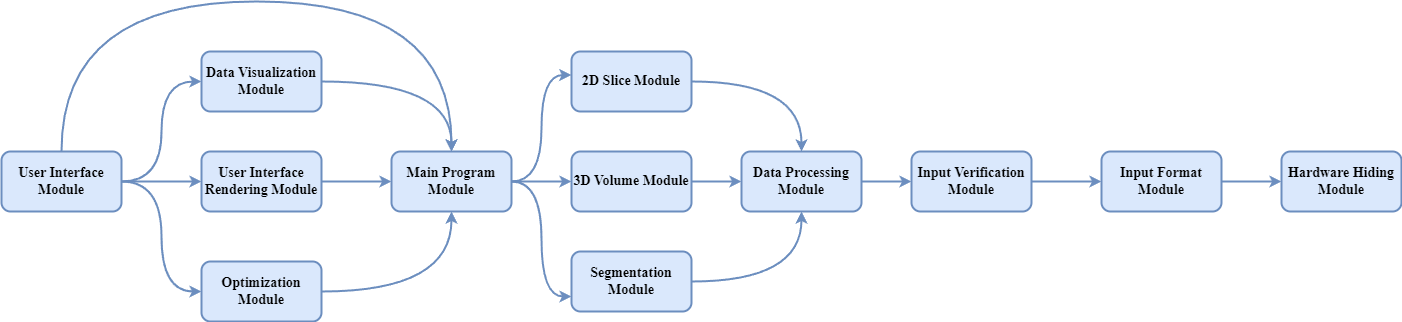
\includegraphics[width=\textwidth]{ModuleHier-Final.png}
  \caption{Use hierarchy among modules}
  \label{FigUH}
\end{figure}

%\section*{References}

% \section{User Interfaces}

% \wss{Design of user interface for software and hardware.  Attach an appendix if
%   needed. Drawings, Sketches, Figma}

% \section{Design of Communication Protocols}

% \wss{If appropriate}

% \section{Timeline}

% \wss{Schedule of tasks and who is responsible}

% \wss{You can point to GitHub if this information is included there}

\newpage
\bibliographystyle {plainnat}
\bibliography{../../../refs/ReferencesMG}

\newpage{}

\end{document}